\documentclass[fleqn,10pt]{olplainarticle}
% Use option lineno for line numbers 
\usepackage{float}
\usepackage{graphicx}
\usepackage[backend=biber,style=ieee,sorting=none]{biblatex}
\addbibresource{sample.bib}

\title{Evaluating Model Compilation for TinyML: A Case Study Using ONNX and TVM}

\author[1]{First Author}
\author[2]{Second Author}
\affil[1]{Address of first author}
\affil[2]{Address of second author}

\keywords{TinyML, ONNX, Apache TVM, Model Compilation, Edge Deployment}

\begin{document}

\flushbottom
\maketitle

\begin{abstract}
This work investigates how model compilation affects a small neural network intended for resource-constrained deployment. A LeNet-style convolutional neural network is trained on MNIST, exported to ONNX, and compiled using Apache TVM for CPU execution. The ONNX and TVM versions are compared in terms of accuracy, model size, graph structure, and inference performance. The results show that TVM preserves the model output, but does not make the model smaller or faster in this setup. The TVM artifacts are larger because they include a compiled kernel library, and the CPU performance is worse than ONNX Runtime without hardware-specific tuning. The main finding is that compilation changes the representation of the model, but additional techniques such as quantization or target-specific tuning are needed to improve size or speed.
\end{abstract}

\thispagestyle{empty}
\section{Introduction}

Machine learning is increasingly being deployed on resource-constrained edge devices, such as microcontrollers and low-power embedded systems \cite{banbury2020tinyml}. These environments impose strict limitations on memory, compute capability, and energy consumption, making deployment significantly more challenging than model training. In practice, models might fail to be deployed not due to insufficient accuracy, but because they exceed system constraints. In addition to compute and memory constraints, model size also affects deployment aspects such as over-the-air (OTA) updates over low-bandwidth communication links.

To bridge the gap between training and deployment, models are typically transformed using compilation frameworks. These frameworks convert high-level model representations into optimized forms suitable for execution on target platforms. However, the effects of this transformation process are often not well understood, particularly in terms of how model structure, compute requirements, and memory usage are altered.

This project investigates the impact of model compilation on small neural networks intended for edge deployment. A baseline model is represented using Open Neural Network Exchange (ONNX) \cite{onnx}, and the Apache TVM \cite{chen2018tvm} compiler is used to generate a compiled version. The study compares the model before and after compilation in 32-bit floating-point (FP32) form, focusing on changes in model size, operator structure, and inference performance. Lower-precision (INT8) variants are out of scope and are discussed only as a direction for future work.

The main contribution of this work is a structured analysis of how compilation transforms neural network models at the graph level and how these transformations affect their suitability for deployment in resource-constrained environments. The results provide insight into the role of compilation in bridging the gap between trained models and deployable systems.

\section{Background}

\subsection{Model Compilation}

Model compilation refers to the process of transforming a trained machine learning model into a form that can be efficiently executed on a specific hardware platform. While models are typically developed and trained in high-level frameworks such as PyTorch \cite{paszke2019pytorch} or TensorFlow \cite{abadi2016tensorflow}, these representations are not directly suitable for deployment, especially in resource-constrained environments.

The compilation process bridges this gap by converting the model into an optimized representation. This involves modifying the computational graph, for example by reorganizing operations or combining multiple operators into a single operation (operator fusion). Such transformations can reduce memory access, improve data locality, and simplify execution.

In addition to structural changes, compilation also translates high-level operations into lower-level instructions that can be executed efficiently by the target hardware. This step enables models defined in abstract, framework-specific formats to run in a practical deployment setting.

\subsection{Quantization}

Quantization is a technique used to reduce the computational and memory requirements of neural networks by representing numerical values with lower precision \cite{jacob2018quantization}. In most deep learning models, parameters and activations are stored as FP32 values. Quantization converts these values to lower-precision formats, such as INT8.

This reduction in precision decreases model size and can improve computational efficiency, as integer operations are typically faster and require less memory than floating-point operations. As a result, quantization is commonly used in deployment scenarios where resources are limited.

However, quantization may introduce approximation errors, which can affect model accuracy. Quantization is included here as background because it is one of the standard techniques for reducing model size on resource-constrained targets; it is not part of the experimental pipeline in this project, but is discussed as future work.

\subsection{ONNX}
ONNX is an open standard for representing machine learning models in a framework-independent format. It enables interoperability between different deep learning frameworks by providing a common representation that can be shared across tools and platforms \cite{onnx}.

In ONNX, a model is represented as a computational graph consisting of nodes and tensors. Nodes correspond to operators (e.g., convolution, activation functions), while tensors represent data flowing between these operators \cite{onnx}. This graph-based structure makes it possible to analyze model architecture, operator composition, and data dependencies in a standardized way.

ONNX is commonly used as an intermediate representation in deployment pipelines. Models trained in frameworks such as PyTorch or TensorFlow can be exported to ONNX, after which they can be processed by other tools, including compilers and runtime environments. This separation between model development and deployment enables flexibility and portability across different hardware targets.

In this project, ONNX is used as the baseline representation of the neural network prior to compilation. It provides a consistent and framework-neutral view of the model, allowing direct comparison with the compiled version generated by the TVM compiler.

\subsection{Apache TVM}
Apache TVM is an open-source machine learning compiler framework designed to optimize and deploy models across a wide range of hardware platforms \cite{chen2018tvm}. It enables the transformation of high-level model representations, such as ONNX graphs, into efficient executable code tailored to a specific target.

TVM operates by applying a series of compilation and optimization steps to a model’s computational graph. These steps include graph-level transformations, such as operator fusion and simplification, as well as lower-level optimizations that improve execution efficiency \cite{chen2018tvm}. Operator fusion, for example, combines multiple consecutive operations into a single operation, reducing memory access overhead and improving performance.

In addition to modifying the model graph, TVM converts high-level operations into simpler, lower-level instructions that can be executed efficiently on the target hardware. This makes it possible to run models that were originally defined in high-level frameworks in an optimized way \cite{chen2018tvm}. Unlike runtime frameworks that execute models directly, TVM focuses on compilation ahead of execution. This makes it particularly relevant for deployment in resource-constrained environments, where efficient use of memory and compute resources is critical.

In this project, TVM is used to compile ONNX models into optimized representations. The compiled models are analyzed and compared with their original ONNX counterparts to understand how compilation transforms model structure, operator composition, and computational characteristics.

\newpage
\section{Method}

\subsection{Model}
A LeNet-style \cite{lecun1998gradient} convolutional neural network (CNN) was considered suitable due to its simplicity, interpretability, and relevance for lightweight image classification tasks. The model is intentionally kept simple to ensure that the analysis focuses on compilation effects rather than model complexity. The architecture consists of a small number of convolutional and fully connected layers suitable for image classification tasks.

\subsection{Experimental Pipeline}

The experimental pipeline follows a structured transformation from a trained model to a compiled representation:

\begin{enumerate}
    \item Define or load a trained CNN model in PyTorch
    \item Export the model to ONNX format
    \item Inspect the ONNX model as the baseline representation
    \item Compile the ONNX model using Apache TVM
    \item Extract and analyze the compiled model representation
\end{enumerate}

This pipeline enables a direct comparison between the model before and after compilation.

\subsection{Metrics}

The analysis focuses on the following metrics:

\begin{itemize}
    \item \textbf{Model size:} The on-disk size of the serialized model and any associated artifact files, used as an indicator of storage requirements.
    \item \textbf{Operator count:} The number of operators in the computational graph in each representation (ONNX, Relay, and the compiled TVM graph).
    \item \textbf{Operator transformations:} Changes in graph structure between representations, such as operator splits, constant folding, and added executor bookkeeping nodes.
    \item \textbf{Inference performance:} Per-sample latency and throughput at batch size~1 on the CPU host, measured for the ONNX baseline (via ONNX Runtime) and for the TVM-compiled model.
\end{itemize}

In addition, a simple accuracy evaluation is performed to verify that compilation does not significantly affect model correctness.

\subsection{Comparison Setup}

The ONNX model is used as the baseline representation, while the TVM-compiled model represents the optimized version. The model is studied in its FP32 form only; INT8 quantization would require a separate calibration step and is left as future work. The comparison focuses on identifying differences in model structure and computational characteristics between the two representations.

All experiments are conducted on a CPU-based environment, and the results are interpreted qualitatively rather than as hardware-specific performance measurements.

\section{Results}

All measurements below were taken on the same CPU host. The model is the FP32 LeNet-style network trained on MNIST \cite{lecun1998mnist}, and TVM was invoked with target \texttt{llvm} and \texttt{opt\_level=3}; the compile step took 1.69~s. Accuracy is reported on the full MNIST test set (10{,}000 samples), and latency was measured at batch size 1 with 200 timed runs after 10 warm-up runs.

\subsection{Correctness Verification}

PyTorch, ONNX Runtime, and the TVM-compiled model all reach the same top-1 accuracy of 0.9852 on MNIST (Table~\ref{tab:accuracy}, Figure~\ref{fig:accuracy}). Equal accuracy only checks that argmax predictions agree, so we also compared the raw logits coming out of ONNX Runtime and TVM on identical inputs.

\begin{table}[H]
\centering
\caption{Top-1 accuracy on the MNIST test set (10{,}000 samples) for the PyTorch reference model, the exported ONNX model executed with ONNX Runtime, and the TVM-compiled model.}
\label{tab:accuracy}
\begin{tabular}{lc}
\hline
Runtime & Test accuracy \\
\hline
PyTorch & 0.9852 \\
ONNX Runtime & 0.9852 \\
TVM (\texttt{llvm} target) & 0.9852 \\
\hline
\end{tabular}
\end{table}

The maximum absolute difference across the 10{,}000 test samples was $6.68 \times 10^{-6}$ and the mean absolute difference $7.32 \times 10^{-7}$. That is FP32 round-off, not a behavioural change. Top-1 predictions also matched on every single sample (prediction match rate $1.0$, zero mismatches). At the precision the model itself uses, TVM does not change what the network computes.

\begin{figure}[H]
\centering
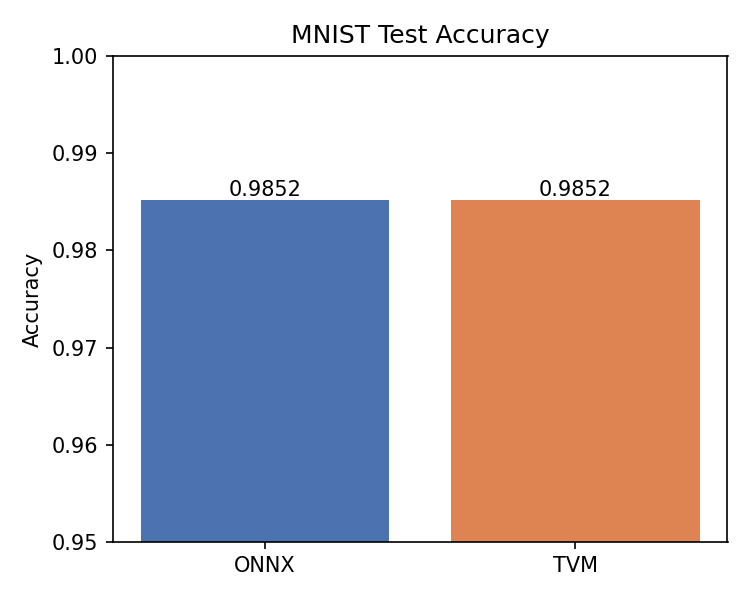
\includegraphics[width=0.55\linewidth]{artifacts/figures/accuracy_comparison.png}
\caption{Top-1 MNIST test accuracy for the ONNX Runtime baseline and the TVM-compiled model. The two bars are visually indistinguishable because both runtimes achieve the same accuracy of 0.9852 on all 10{,}000 test samples.}
\label{fig:accuracy}
\end{figure}

\subsection{Model Size Comparison}

Table~\ref{tab:size} lists every file the two pipelines wrote to disk. ONNX export produces a graph file (20{,}869~B) plus an external weights blob (246{,}696~B), so the ONNX representation totals 267{,}565~B, around 261~KB. TVM compilation produces four files --- a compiled kernel library, a graph JSON, the serialized parameters, and a Relay text dump --- totalling 509{,}036~B, around 497~KB.

\begin{table}[H]
\centering
\caption{On-disk size of the ONNX model and the TVM compilation artifacts.}
\label{tab:size}
\begin{tabular}{lr}
\hline
Artifact & Size (bytes) \\
\hline
ONNX graph (\texttt{lenet\_mnist.onnx}) & 20{,}869 \\
ONNX external data (\texttt{lenet\_mnist.onnx.data}) & 246{,}696 \\
ONNX total & 267{,}565 \\
\hline
TVM compiled library (\texttt{.tar}) & 250{,}603 \\
TVM graph JSON (\texttt{.json}) & 7{,}712 \\
TVM parameters (\texttt{.bin}) & 247{,}652 \\
TVM Relay text (\texttt{.txt}) & 3{,}069 \\
TVM total & 509{,}036 \\
\hline
\end{tabular}
\end{table}

Comparing only the totals would hide what is actually going on in the breakdown. The parameter blobs on the two sides are within a percent of each other (246{,}696~B vs 247{,}652~B), which makes sense: they hold the same FP32 weights, just packaged a little differently. The reason the TVM total is roughly 1.9$\times$ larger is the 250{,}603~B kernel library, which has no counterpart on the ONNX side. ONNX is a pure graph description, and it relies on whichever runtime loads it to produce executable code at use time; TVM produces that executable code ahead of time and ships it inside the artifact. Figure~\ref{fig:size} shows the same comparison graphically.

\begin{figure}[H]
\centering
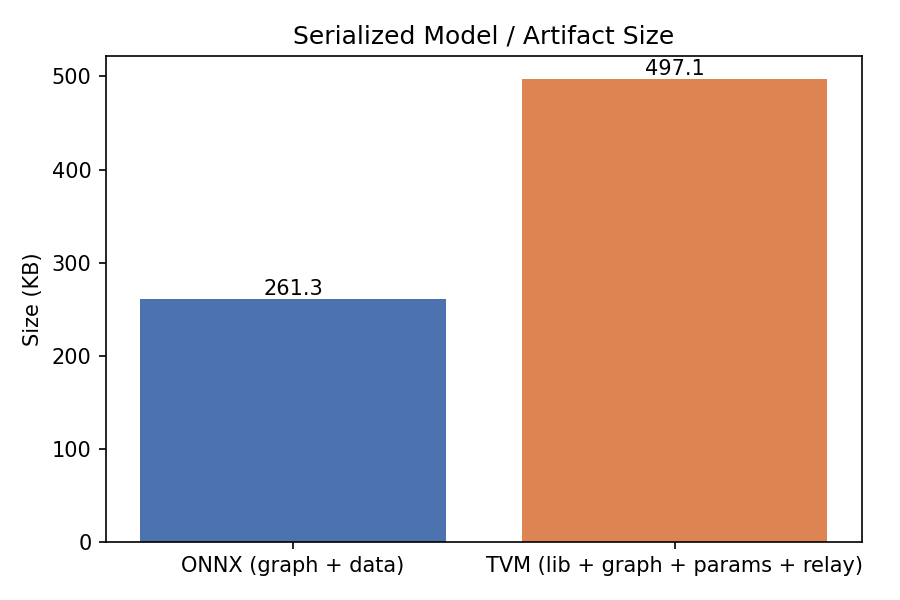
\includegraphics[width=0.6\linewidth]{artifacts/figures/model_size_comparison.png}
\caption{Total on-disk size of the ONNX representation (graph file plus external weight file) and the TVM compilation artifacts (compiled library, graph JSON, parameters, and Relay text). The TVM total is approximately 1.9$\times$ larger than the ONNX total because it additionally contains a compiled kernel library, which the ONNX exchange format does not include.}
\label{fig:size}
\end{figure}

\subsection{Graph and Operator Structure Comparison}

Table~\ref{tab:graph-structure} compares the size of the model description across the three representations, and Table~\ref{tab:onnx-ops} breaks the ONNX side down by operator type. Figure~\ref{fig:onnx-graph} shows the ONNX graph itself, and Figure~\ref{fig:relay} shows the corresponding Relay program with the inline type annotations stripped for readability.

\begin{table}[H]
\centering
\caption{Graph-level structure of the model in its ONNX, Relay, and TVM-compiled forms.}
\label{tab:graph-structure}
\begin{tabular}{lc}
\hline
Representation & Count \\
\hline
ONNX graph nodes & 14 \\
Relay calls (after ONNX import) & 17 \\
Relay text lines & 25 \\
TVM compiled graph nodes & 20 \\
TVM graph argument nodes & 11 \\
\hline
\end{tabular}
\end{table}

\begin{table}[H]
\centering
\caption{Operator-type counts in the exported ONNX graph.}
\label{tab:onnx-ops}
\begin{tabular}{lc}
\hline
Operator & Count \\
\hline
AveragePool & 2 \\
Concat & 1 \\
Conv & 2 \\
Gemm & 3 \\
Relu & 4 \\
Reshape & 1 \\
Shape & 1 \\
\hline
Total & 14 \\
\hline
\end{tabular}
\end{table}

Looking only at the counts, the somewhat surprising thing is that they grow rather than shrink along the pipeline: 14 ONNX nodes, then 17 Relay calls, then 20 nodes in the compiled TVM graph (the 11 argument nodes are the model input plus the constant parameter tensors). Compilation is usually associated with fusion and simplification, so this needs a small explanation, which is easiest to give once the actual representations have been shown.

\begin{figure}[H]
\centering
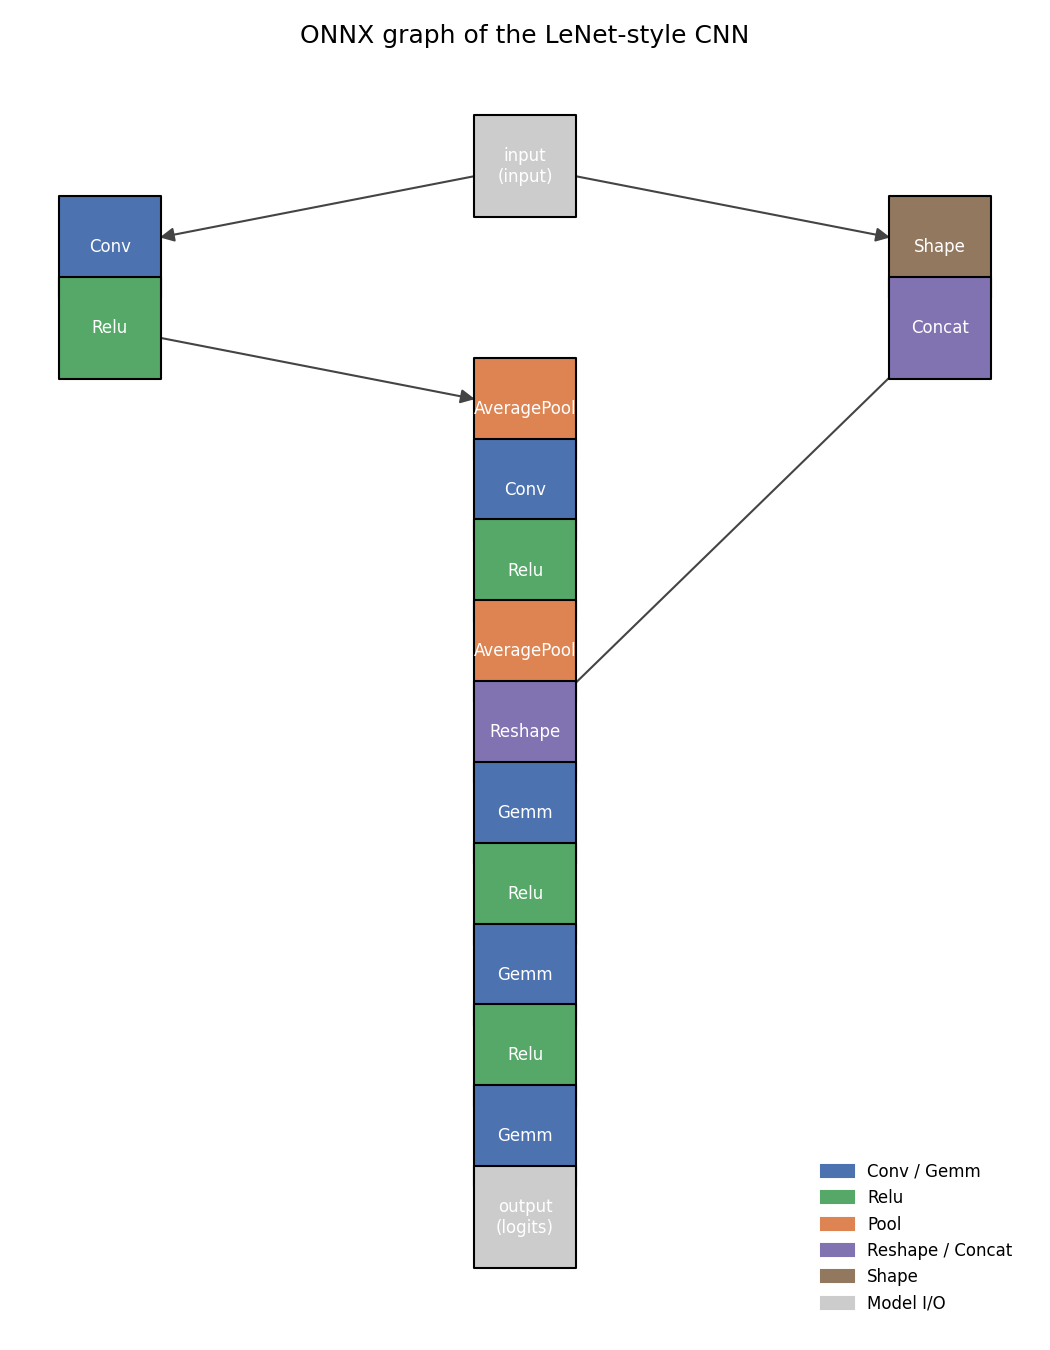
\includegraphics[width=0.55\linewidth]{artifacts/figures/onnx_graph.png}
\caption{Visualization of the exported ONNX graph, rendered with the Netron model viewer \cite{roeder_netron}. The main computational path runs top-to-bottom (Conv $\rightarrow$ Relu $\rightarrow$ AveragePool $\rightarrow$ Conv $\rightarrow$ Relu $\rightarrow$ AveragePool $\rightarrow$ Reshape $\rightarrow$ three Gemm$/$Relu pairs $\rightarrow$ logits). A small Shape$/$Concat side branch supplies the dynamic shape tensor consumed by Reshape; this pattern is introduced by the PyTorch-to-ONNX exporter rather than by the model itself.}
\label{fig:onnx-graph}
\end{figure}

The Relay step in Figure~\ref{fig:relay} is the easier one to read off: each ONNX \texttt{Conv} has been turned into \texttt{nn.conv2d} followed by \texttt{nn.bias\_add}, and each ONNX \texttt{Gemm} into \texttt{nn.dense} followed by \texttt{add}. That alone contributes five new calls. At the same time, the \texttt{Shape} and \texttt{Concat} nodes from the ONNX graph are gone: the importer constant-folded the dynamic-reshape subgraph into a literal \texttt{newshape=[1, 400]} once the input shape was fixed, removing two nodes. Net effect: $14 + 5 - 2 = 17$, which is what Table~\ref{tab:graph-structure} reports. The further jump from 17 Relay calls to 20 TVM graph nodes is not new computation; the extra three nodes are bookkeeping introduced by the graph executor (entry points for the input and the constant parameter tensors), not arithmetic. None of these counts says anything about how much work the model does at inference time --- they describe how the program is written down in each representation, which is a different thing.

\begin{figure}[H]
\begin{verbatim}
def @main(%input: Tensor[(1, 1, 28, 28), float32])
        -> Tensor[(1, 10), float32] {
  %0  = nn.conv2d(%input, W0, padding=[2,2,2,2],
                  channels=6, kernel_size=[5, 5]);
  %1  = nn.bias_add(%0, b0);
  %2  = nn.relu(%1);
  %3  = nn.avg_pool2d(%2, pool_size=[2,2], strides=[2,2],
                      padding=[0,0,0,0], count_include_pad=True);
  %4  = nn.conv2d(%3, W1, padding=[0,0,0,0],
                  channels=16, kernel_size=[5, 5]);
  %5  = nn.bias_add(%4, b1);
  %6  = nn.relu(%5);
  %7  = nn.avg_pool2d(%6, pool_size=[2,2], strides=[2,2],
                      padding=[0,0,0,0], count_include_pad=True);
  %8  = reshape(%7, newshape=[1, 400], allowzero=True);
  %9  = nn.dense(%8, W2, units=120);
  %10 = add(%9, b2);
  %11 = nn.relu(%10);
  %12 = nn.dense(%11, W3, units=84);
  %13 = add(%12, b3);
  %14 = nn.relu(%13);
  %15 = nn.dense(%14, W4, units=10);
  add(%15, b4)
}
\end{verbatim}
\caption{TVM Relay program produced by the ONNX-to-Relay importer for the LeNet-style CNN. Inline type annotations and span comments have been removed, and constant-tensor references have been renamed (\texttt{W0}\dots\texttt{W4}, \texttt{b0}\dots\texttt{b4}) for readability. The full Relay text is available in \texttt{artifacts/tvm/lenet\_mnist\_relay.txt}.}
\label{fig:relay}
\end{figure}

\subsection{Performance Comparison}

On the same CPU host, ONNX Runtime ran at a mean of 0.048~ms per sample (median 0.043~ms, P95 0.050~ms, throughput 20{,}874.7 samples/s) and the TVM-compiled model ran at a mean of 2.349~ms (median 0.179~ms, P95 14.023~ms, throughput 425.8 samples/s); see Table~\ref{tab:performance} and Figure~\ref{fig:latency}.

\begin{table}[H]
\centering
\caption{Single-sample inference latency and throughput on CPU for ONNX Runtime and the TVM-compiled model (batch size 1, 200 timed runs after 10 warm-up runs).}
\label{tab:performance}
\begin{tabular}{lcccc}
\hline
Runtime & Mean (ms) & Median (ms) & P95 (ms) & Throughput (samples/s) \\
\hline
ONNX Runtime & 0.048 & 0.043 & 0.050 & 20{,}874.7 \\
TVM (\texttt{llvm} target) & 2.349 & 0.179 & 14.023 & 425.8 \\
\hline
\end{tabular}
\end{table}

TVM is slower on every statistic. At the median the gap is about $4.2\times$, but at the mean it widens to roughly $49\times$, driven almost entirely by a P95 of 14.023~ms against ONNX Runtime's 0.050~ms. A median that is close to ONNX paired with a P95 that is two orders of magnitude higher does not look like uniform slowness; it looks like a few outlier runs pulling the mean upwards. With no autotuning, default schedules, and a small network at batch size 1, these results should not be interpreted as the best performance TVM can achieve on this workload.

\begin{figure}[H]
\centering
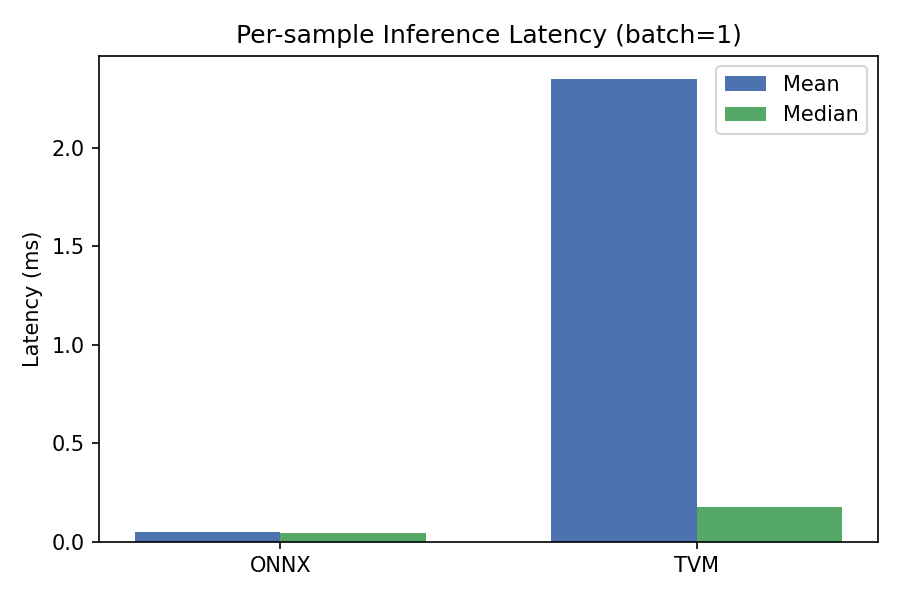
\includegraphics[width=0.65\linewidth]{artifacts/figures/latency_comparison.png}
\caption{Per-sample inference latency at batch size 1 for ONNX Runtime and the TVM-compiled model, reported as both mean and median over 200 timed runs. The gap between the TVM mean (2.349~ms) and median (0.179~ms) reflects a heavy-tailed latency distribution; ONNX Runtime is faster on both statistics in this configuration.}
\label{fig:latency}
\end{figure}

\section{Discussion}

Read together, the results say something fairly simple. TVM kept the model's behaviour intact (same predictions, same logits up to FP32 noise), but at this scale and on this hardware the compiled model was neither smaller nor faster than the ONNX baseline. The rest of this section is about why that happened, and what it does and does not say about model compilation as a deployment strategy.

\subsection{Why the TVM artifacts are not smaller than the ONNX model}

One way to see why TVM did not shrink the model is to look at what is actually inside each artifact. ONNX is an exchange format: a graph description plus the parameters, nothing else. TVM, by contrast, is an ahead-of-time compiler, so its output adds a compiled kernel library on top of the graph and the parameters. Table~\ref{tab:size} shows this directly: the parameter blobs are within a percent of each other (246{,}696~B vs 247{,}652~B), and the entire size gap comes from the 250{,}603~B compiled library, which has no counterpart on the ONNX side.

Compilation alone cannot reduce the model size. It does not remove parameters, it does not change their precision, and it adds an executable that was not present in the ONNX file. Reducing the model size requires a different kind of transformation, such as quantization, pruning, or weight sharing, that operates on the parameter payload itself. TVM is a compiler, not a compression tool, and the size result is consistent with that.

\subsection{Why the TVM-compiled model is slower than ONNX Runtime here}

The slowdown also lines up with what TVM is, and is not, being asked to do here. The setup is a tiny CNN, batch size 1, generic CPU, no autotuning, default schedules. Three things matter under those conditions.

ONNX Runtime is a strong baseline. It ships hand-tuned CPU kernels for exactly the operators in this model (\texttt{Conv}, \texttt{Gemm}, \texttt{AveragePool}, \texttt{Relu}), and on the CPU host used in this experiment it is already highly optimized, so a framework that wants to beat it needs to bring something specific. TVM, in contrast, was used at \texttt{opt\_level=3} with the default schedules for the \texttt{llvm} target. The performance numbers reported for TVM in the literature usually come from operator-level autotuning (AutoTVM, Ansor) \cite{zheng2020ansor} on the actual target hardware, and we did neither, so these results should not be interpreted as the best performance TVM can achieve. The third issue is workload size: a LeNet at batch size 1 finishes in tens of microseconds, and at that scale the per-call overhead of the TVM graph executor --- allocating temporaries, dispatching kernels, walking the graph --- becomes a meaningful fraction of the total. The heavy-tailed shape of the TVM latencies (median 0.179~ms, P95 14.023~ms) is consistent with this: most calls finish quickly and a small number of outliers pull the mean up.

In other words, the performance numbers are not a general statement about TVM versus ONNX Runtime. They describe what happens when a microsecond-scale workload is run through a compiler that has not been tuned for the host and that has its own per-call overhead.

\subsection{Why the graph node count can grow rather than shrink after compilation}

The progression $14 \rightarrow 17 \rightarrow 20$ in Table~\ref{tab:graph-structure} can look counter-intuitive at first, since compilation is usually associated with fusion and simplification. The reason the count grows is that each step uses a slightly different set of operators to describe the same model. Going from ONNX to Relay, the importer expands ONNX operators that bundle several primitives (\texttt{Conv} into \texttt{conv2d + bias\_add}, \texttt{Gemm} into \texttt{dense + add}) and at the same time folds the dynamic-shape subgraph (\texttt{Shape}, \texttt{Concat}) into a constant. The split adds operators, the fold removes them, and the net is $+3$. Going from Relay to the TVM executor graph, the further $+3$ are not new computation either; they are routing nodes that the executor adds for its own bookkeeping --- entry points for the input and for the constant parameter tensors, not arithmetic.

In other words, the node counts in Table~\ref{tab:graph-structure} are a property of how each representation is written down, not of how much work the model does at inference time. The ONNX count of 14 is also not the smallest possible description.

\subsection{What compilation actually changed in this experiment}

Taken together, the size, structure and performance results indicate that TVM changed the form of the artifact rather than what the artifact does. Inputs and outputs match to within FP32 round-off (max absolute logit difference $6.68 \times 10^{-6}$, zero prediction mismatches in 10{,}000 samples), the parameter blob is the same up to serialization, and the operator semantics are unchanged by construction. The main new part of the TVM output is the compiled kernel library: the artifact is no longer an exchange description that some other runtime needs to interpret, but an executable bundle that the TVM runtime can run directly. This is the deployment-relevant change. The size, structure and latency numbers in the Results section can be understood as side effects of that change of form, rather than as the main result.

\subsection{Implications for stronger deployment gains}

The TinyML scenarios that motivate this kind of pipeline --- microcontrollers, low-bandwidth OTA updates, tight power envelopes --- usually need much more than a change of artifact form. Turning the workflow studied here into something that would actually pay off on a real edge device would require at least two further steps.

The first is quantization, for instance to INT8. Table~\ref{tab:size} already shows that the parameter blob is the dominant contributor to size on both sides, and quantization is the transformation that goes after exactly that, with the additional benefit of cheaper inference on hardware with good integer support. The second is hardware-specific tuning, either by autotuning the TVM kernels (AutoTVM, Ansor) for the actual deployment target, or by cross-compiling to that target instead of using the generic \texttt{llvm} CPU target used here.

Without at least one of those, an out-of-the-box ONNX-to-TVM pipeline preserves correctness and changes the form of the artifact, but does not in itself make the model smaller or faster.

\section{Conclusion}

This project compared an ONNX baseline against a TVM-compiled version of the same LeNet-style CNN on MNIST, focusing on accuracy, model size, graph structure, and inference latency on a CPU host. The compiled model preserves predictions and logits to within FP32 round-off, but in this configuration it is not smaller or faster than the ONNX baseline executed with ONNX Runtime: the TVM artifacts are roughly $1.9\times$ larger because they include a compiled kernel library, and inference latency at batch size 1 is higher with default schedules and no autotuning.

The practical takeaway is that an out-of-the-box ONNX-to-TVM pipeline is best understood as a change of representation rather than as an automatic optimization. Reducing model size or inference latency for real edge deployment would require additional steps beyond compilation: quantization (for example to INT8) to operate directly on the parameter payload, and either autotuning or cross-compilation to a specific embedded target instead of the generic \texttt{llvm} CPU target used here. Both are natural directions for future work, but were out of scope for this project.

\newpage
\printbibliography


\end{document}